%!TEX root = report.tex
This section presents the results of the experiments with the one- and two- dimensional model discussed in \cref{s:experiment}, in \cref{ss:results:1D} and \cref{ss:results:2D}, respectively.

\subsection{One-Dimensional Model}
\label{ss:results:1D}
	\Crefrange{tab:results:1D:10:1000}{tab:results:1D:1000:10000} in \cref{a:results1D} present the results of the experiment with the one dimensional model. The average accuracies, without the $\pm \infty$ are presented in \cref{tab:results:1D:averageAccuracies}.

	In \cref{tab:results:1D:10:1000,tab:results:1D:10:10000} we observe that the accuracy of the 1D simulation is reasonable for temperatures greater than 0.4. In the simulation with $\numberOfSpins = 10$. 
	%
	The simulation with $\numberOfSpins = 100$ starts being accurate at $\temperature = 1.4$ if $\numberOfSamples = 1000$ and at $\temperature = 0.8$ if $\numberOfSamples = 10000$. 
	%
	If we increase the number of spins to $\numberOfSpins = 1000$ we only find reasonable accuracy with $\numberOfSamples = 10000$ for $\temperature > 1.6$.

	For all values of $\numberOfSpins$ we find that the accuracy improves we find that the accuracy improves as the number of samples increases. 

	\begin{table}
		\centering
		\caption{Average accuracies of the one-dimensional simulation.}
		\begin{tabular}{
			S[table-number-alignment = center]
			S[table-format = 1.3, round-mode=places, round-precision=3, table-number-alignment = center]
			S[table-format = 1.3, round-mode=places, round-precision=3, table-number-alignment = center]
			S[table-format = 1.3, round-mode=places, round-precision=3, table-number-alignment = center]}
			\toprule
			~ & \multicolumn{3}{c}{Number of Spins (\numberOfSpins)}\\ 
			\cmidrule(r){2-4}
			\numberOfSamples & 10 & 100 & 1000 \\
			 \midrule 
			 1000 & -0.848369 	& -1.115464 & -0.095644\\
			 1000 & 0.873160 	& 0.813785 	& 0.726252\\
			\bottomrule
		\end{tabular}
		\label{tab:results:1D:averageAccuracies}			
	\end{table}

\subsection{Two-Dimensional Model}
\label{ss:results:2D}
	The average energy, specific heat and average magnetization per spin for the different combinations of \numberOfSpins and \numberOfSamples can be found in \cref{fig:results:2D}. 

	In \cref{fig:results:2D:averageEnergy} we observe that the average energy per spin is hardly influenced by the number of samples for $\numberOfSamples = 10$. As the number of spins in the simulation increases, the difference between the simulation with $\numberOfSamples = \num{1.e+3}$ and $\numberOfSamples = \num{1.e+4}$ increases. In general we observe that the average energy per spin increases as the temperature increases. In \cref{eq:experiment:1D:averageEnergy} the phase transition that we expect at $\criticalTemperature \approx \num{2.2}$ is indicated by an increase in the average energy per spin, after $\rfrac{\averageEnergy}{\numberOfSpins}$ has been constant for $\temperature << \criticalTemperature$. 

	In \cref{fig:results:2D:specificHeat} we observe a bell-shaped curve in the specific heat per spin around $\temperature = 2$. The curve is more defined when $\numberOfSamples$ is higher and when the number of spins in the simulation increases. The highest points of these bell curves are found near $\temperature = \criticalTemperature$, \ie at the phase transition.

	Comparing the measured average magnetization per spin in \cref{fig:results:2D:averageMagnetization} with the theoretical value in the same figure we observe that the curves reflecting the results of the simulation are less steep. Furthermore the smaller simulations seem to give a better approximation than the simulation with a lot of spins. In \cref{fig:results:2D:averageMagnetization} the phase transition is clearly illustrated by the theoretical line. Nearly all lines in this figure illustrate that $\rfrac{\magnetization}{\numberOfSpins}$ is positve for low temperatures, it then decreases around $\temperature = \criticalTemperature$ and stays zero for temperatures that are a bit higher than the critical temperature. The last observation only holds for the theoretical infinite system. Most of the simulated systems do not reach $\rfrac{\magnetization}{\numberOfSpins} = 0$.

	\begin{figure}
		\centering
		\begin{subfigure}{\columnwidth}
			\centering
			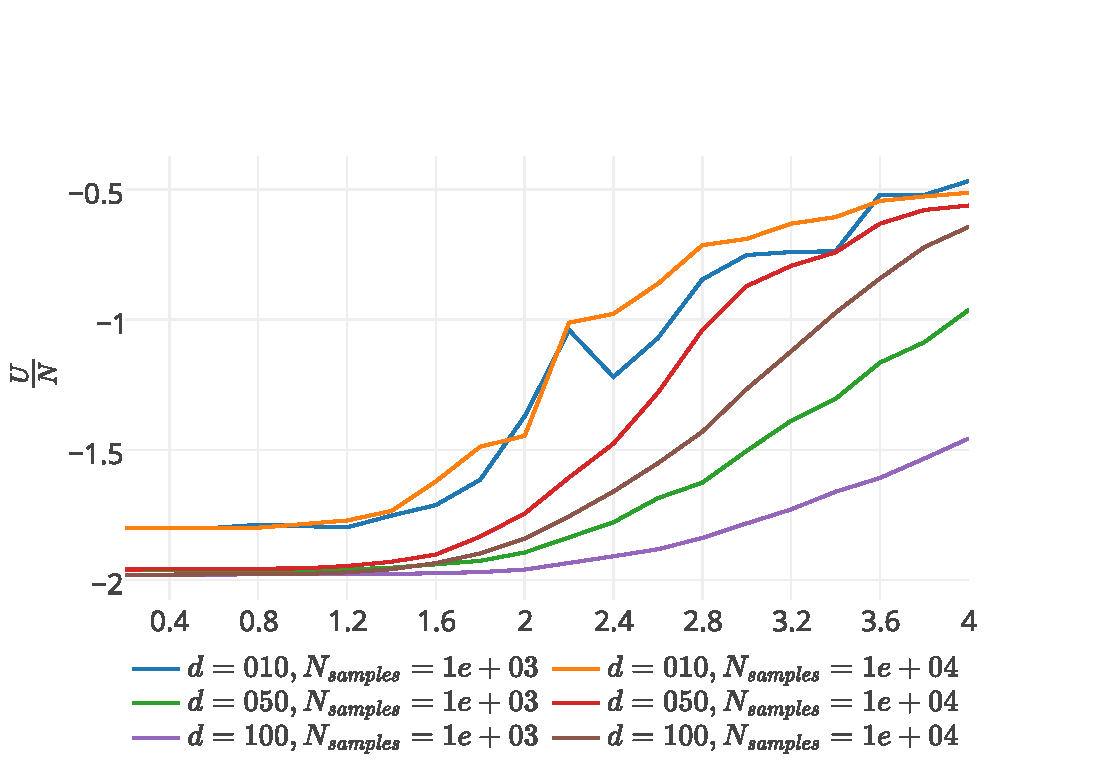
\includegraphics[width=\textwidth]{./img/2D/averageEnergy}
			\caption{Average energy per spin.}
			\label{fig:results:2D:averageEnergy}
		\end{subfigure}
		\begin{subfigure}{\columnwidth}
			\centering
			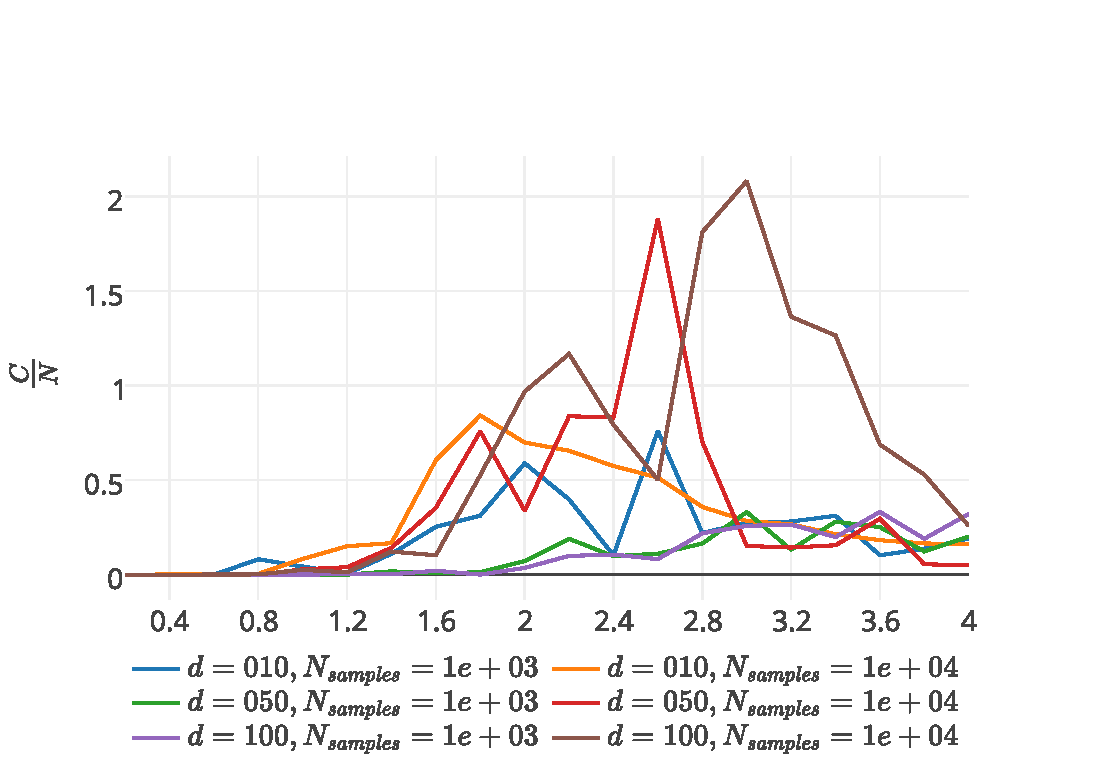
\includegraphics[width=\textwidth]{./img/2D/specificHeat}
			\caption{Specific heat per spin.}
			\label{fig:results:2D:specificHeat}
		\end{subfigure}	
		\begin{subfigure}{\columnwidth}
			\centering
			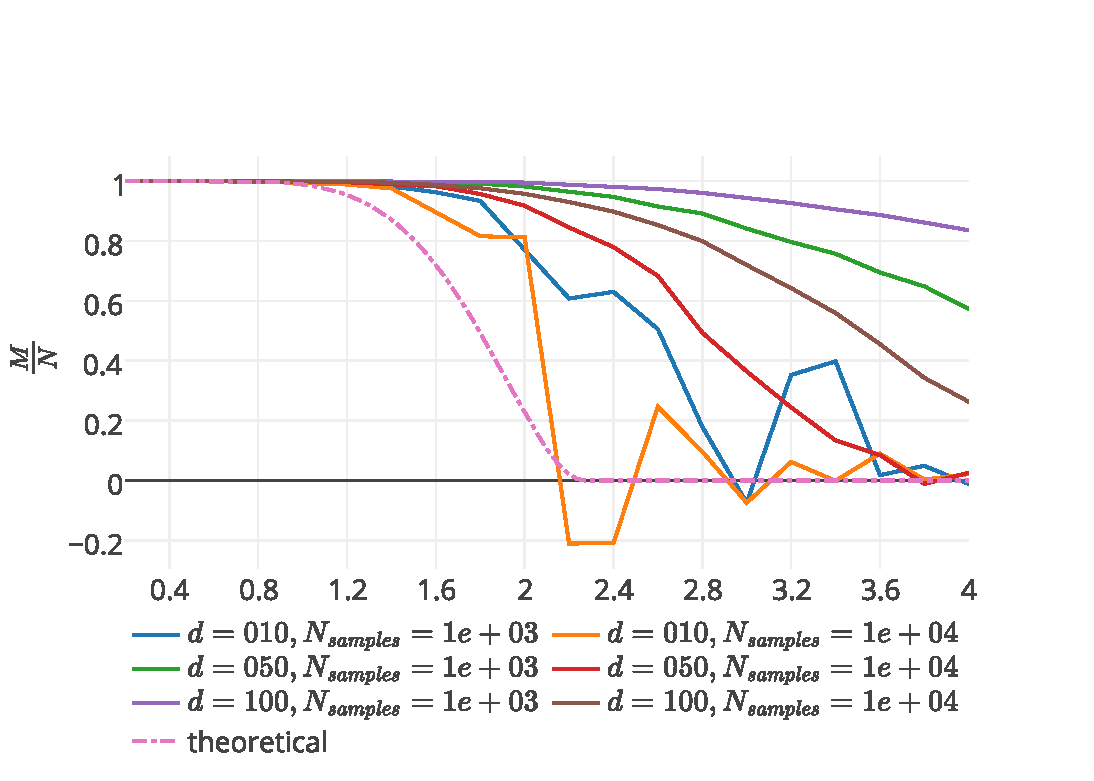
\includegraphics[width=\textwidth]{./img/2D/averageMagnetization}
			\caption{Average magnetization per spin.}
			\label{fig:results:2D:averageMagnetization}
		\end{subfigure}		
		\caption{The \subref{fig:results:2D:averageEnergy} average energy, \subref{fig:results:2D:specificHeat} specific heat and \subref{fig:results:2D:averageMagnetization} average magnetization per spin in a 2D Ising model with $\dimensionality = 10, 50, 100$ and $\numberOfSamples = 1000, 10000$.}
		\label{fig:results:2D}
	\end{figure}